\section{Diseño del circuito} 
\subsection{Esquemático}

Para el diseños de hardware se utilizo el circuito que se muestra en la figura \ref{Fig: Diseño hardware} y en la figura \ref{Fig: Diagrama_hardware} se puede observar el diagrama eléctrico que se siguió. De manera que para la conversión de tensiones de [0V, 9V] a [0V, 3V], por otro lado se utilizo un switch con el fin de controlar la comunicación en \textit{USART}.

\begin{figure}[H]
\centering
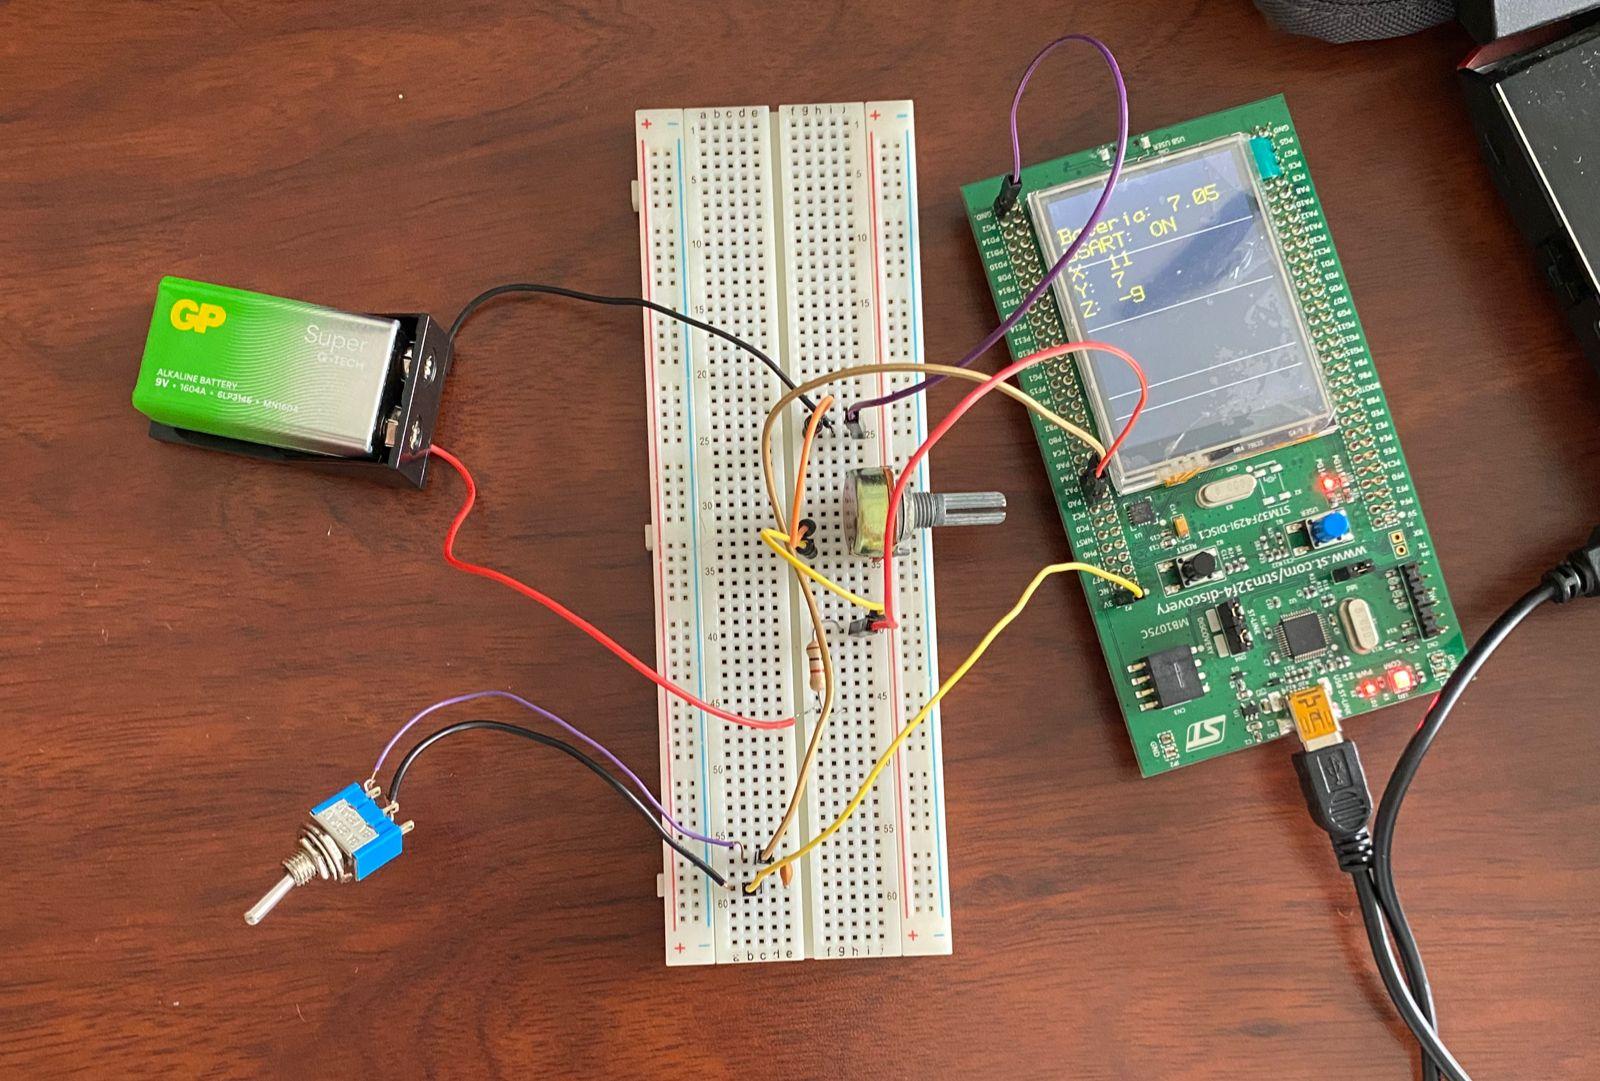
\includegraphics[width=0.9\textwidth]{Imagenes/Circuito.jpg} 
\caption{Diseño del circuito.}
\label{Fig: Diseño hardware}
\end{figure}

\begin{figure}[H]
\centering
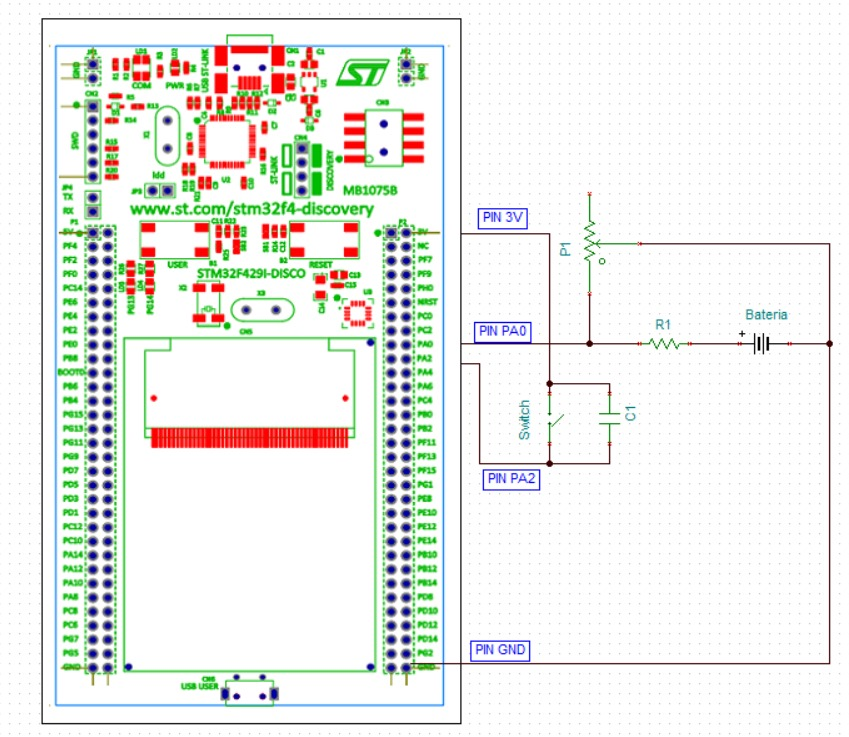
\includegraphics[width=0.9\textwidth]{Imagenes/Diagrama_electricoLab4.jpg} 
\caption{Diagrama Eléctrico del Circuito}
\label{Fig: Diagrama_hardware}
\end{figure}


\subsection{Disminución del efecto rebote de los switches}
De acuerdo con la información de referencia del STM32F429, el microcontrolador tiene resistencias de \it{pull-up} internas de \SI{40}{\kilo\ohm} \cite{stm32micro}.
La obtención de estos valores de resistencias y el valor de la capacitancia se da por medio de la ecuación
\begin{equation}
    \tau = RC.
\end{equation}
Como el interruptor oscila entre estar cerrado y abierto entre diez a cien veces en un periodo de \SI{1}{\milli\second}, se puede llegar a despejar la capacitancia $C$
\cite{boton},
\begin{equation*}
    C = \frac{\tau}{R} = \frac{\SI{1}{\milli\second}}{\SI{40}{\kilo\ohm}} = \SI{25}{\nano\farad}.
\end{equation*}

Por lo tanto, se decide utilizar una capacitancia de \SI{22}{\nano\farad}, ya que es el valor comercial más cercano.
 

 
\subsection{Cálculo de las resistencias}
En la figura \ref{Fig: cal_resist}, se ilustra la red resistiva que ``convierte'' tensiones entre \SI{0}{\volt} a \SI{9}{\volt} a un rango entre \SI{0}{\volt} a \SI{3}{\volt}. Se destaca que a la hora implementarlo, se decidió utilizar un potenciómetro en lugar de la resistencia \textit{$R_2$}, el motivo es porque así se puede manipular la tensión de salida y probar la condición de cuando la tensión llega a valores cercanos a \SI{7}{\volt}. El calculo de las resistencia se observa a continuación
\begin{align}
    V_o &= \frac{R_2 \cdot V_\text{in}}{R_1 + R2}\\
\end{align}
siendo $R_1$ un valor arbitrario. Por lo tanto, para un $R_1 = \SI{1}{\kilo\ohm}$, $R_2$ debe de ser
\begin{align*}
    R_2 &\approx \SI{1250}{\kilo\ohm}.
\end{align*}
Se escogerá un potenciómetro de \SI{5}{\kilo\ohm} que va a sustituir la resistencia $R_2$.

\begin{figure}[H]
\centering
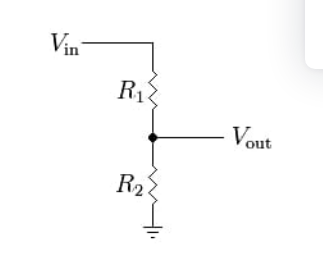
\includegraphics[width=0.6\textwidth]{Imagenes/divisordetension.png} 
\caption{Red resistiva para convertir el rango de la tensión de entrada a un rango apto para el STM32F429. Fuente y créditos: \cite{divisor}.}
\label{Fig: cal_resist}
\end{figure}

